\subsection{Model Results}

\subsubsection{Runtime and Efficiency Analysis}

To evaluate the computational efficiency of the simulation model, a series of runs were performed using increasing ray counts. The aim was to determine how runtime scales with simulation complexity, and whether additional rays meaningfully improve hit accuracy.

\begin{figure}[H]
    \centering
    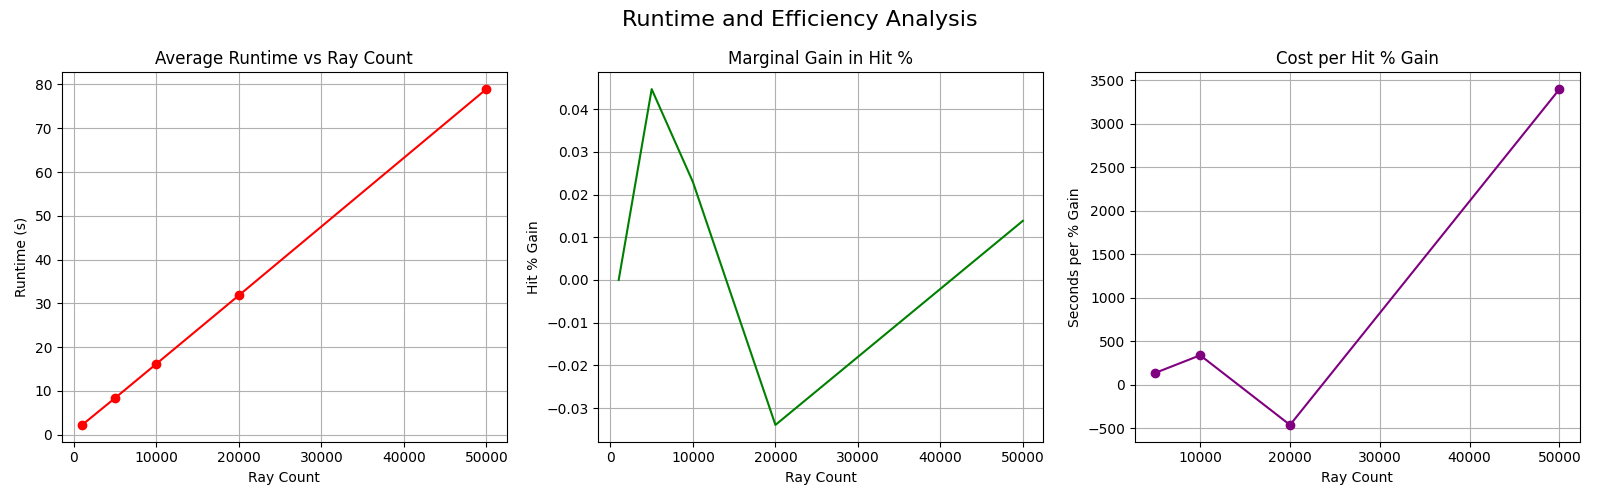
\includegraphics[width=\textwidth]{chapters/methodology/SoftwareModel/images/run time analysis.png}
    \caption{Runtime and efficiency trends with increasing ray count. Left: Runtime increases linearly with ray count. Middle: Marginal gain in hit accuracy. Right: Cost in seconds per 1\% hit gain.}
    \label{fig:runtime_efficiency}
\end{figure}

\textbf{Scalability}: As shown in Figure~\ref{fig:runtime_efficiency} (left), the simulation runtime increases approximately linearly with the number of rays. This behaviour suggests the implementation scales efficiently.

\textbf{Accuracy vs. Rays}: The centre plot illustrates the marginal gain in hit percentage between successive ray counts. Gains were most meaningfully prominent between 20,000 and 50,000 rays.

\textbf{Cost per Gain}: The rightmost plot quantifies computational cost per 1\% gain in accuracy. It reveals that simulations using 50,000 rays are inefficient: they incur high runtimes with negligible improvement. In contrast, ray counts between 10,000 and 20,000 yield the most cost-effective results.

\textbf{Utilisation}: Based on these findings, simulations were conducted using \textbf{15,000 rays} to benefit from the best trade-off between runtime and accuracy.

